\documentclass{article}

\usepackage{graphicx}

\author{Nic Hollingum - 308193415}
\title{Computational Geometry - Assignment 4}

\addtolength{\oddsidemargin}{-.875in}
\addtolength{\evensidemargin}{-.875in}
\addtolength{\textwidth}{1.75in}
\addtolength{\topmargin}{-1in}
\addtolength{\textheight}{2.5in}

\begin{document}
\maketitle

\section {Euclidian Problems}

\subsection*{a}
By the triangle inequality, this is trivial, we shall prove it by contradiction.
We have a cycle of nodes which we vist, and removing nodes from the cycle represents removing elements to form a subset.
Conversely adding nodes represents increasing a subset to the size of the set.
In order for a subset not to be shorter than the superset, then there must exist some superset shorter than its subset.
In other words we have to decrease the length of the cycle by adding a node, or, we stop at some node in the cycle, move to the new node, then back to the next node in the cycle and continue.
But this requires the sum of paths from some node in the cycle to new node, and new node back to next, be less than some node to the next, which violates the triangle inequality (if a, b and c are edges of a triangle, then the length of any 1 must be less than the sum of the other 2).

\subsection*{b}
Proof by example:

\begin{figure}[htb]
\begin{center}
\leavevmode
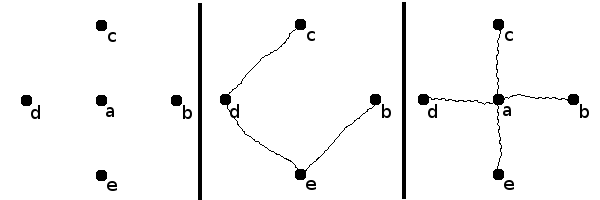
\includegraphics[width=0.6\textwidth]{mst.png}
\end{center}
\end{figure}
\label{fig:mst}

Using the 5 points here, where our subset lacks point $a$, we see that the MST grows longer.
When $a$ is absent, we must choose 3 of the 6 edges in $k_4$, and the 3 shortest edges are those around the perimeter.
Each of the perimeter points is 1 unit up, down, left or right of $a$, and the border edges have length $\sqrt 2$ accordingly, the total length is $3 \sqrt 2 = 4.24$.
When $a$ is present then the MST is 4 edges from $a$ to all of the corner points.
Each corner point is 1 unit distance from $a$, and so the MST has length 4, which is less than above.
Therefore even though the middle graph is a subset of the left, it has a longer MST than the right.

\subsection*{c}
First TSP must be more than MST, this can be verified by a counting problem, and that MST is a tree and TSP is a cycle.
given n points, where each is equidistant from evey other (we need n-1 dimensions to do this by the way) we note that the MST must have n-1 edges and so n-1 length, but the cycle must return to its start node, and so must have n edges and n length.
If the points are not equidistant we know that if the TSP is able to choose a shorter path, the MST is as well, but there are times when the MST can avoid long paths where the TSP cant.
Consider many points spread out evenly along a circle edge, with a gap on one side.
The MST is able to avoid this gap and simply choose the points around the perimeter, wheres at TSP will either take this edge, or backtrack along other edges and so waste time.

We also note that given an MST, we are able to find some repeating cycle, using depth-first search along all branches of the tree.
The salesman starts at some node in the tree and traverses it depth first.
Each edge must be crossed once to go to new nodes, and again later to return prom them, hence exactly twice.
Therefore we have a repeating cycle no more than double the length of the MST which visits every node.
Clearly a more efficient TSP can be contrived by skipping nodes we know we have visited and we will return from.
Such that if we would return from a to b, then b to it's parent c, we simply go from a to c and save the distance, therefore optimal TSP must be less or equal to 2*MST.

\section {Voronoi Convex Hull}

This question can be posed more formally: For which pairs of points can we place an infinitely large circle such that the circle intersects both points and no others.
Clearly such a circle constitutes an unbounded barrier between cells in the Voronoi diagram.
If we can place such a circle then all the points in the triangle between its centre, the radial line joining the centre to one of the points, and a segment meeting the line between both points perpendicular (a right angled triangle) belongs to the cell for that point, and the mirror for the other cell.
Since the circle is infinitely large the area of the triangle can be infinitely large and the region is unbounded.

Furthur there can exist no unbounded cell for which such a circle cannot be constructed.
Consider the unbounded barrier between 2 unbounded cells.
Clearly if a cell is unbounded it must have at least 1 unbounded barrier (though usually 2), and therefore there must be other unbounded cells neighbouring this one.
Where $n=2$ the voronoi diagram is defined but the convex hull is just a line, therefore the result is trivially obvious.
Given we have unbounded barriers we are able to pick a point infinitely far out along the barrier and call this the circle's centre.
Then when we draw the circle no other point in the set will be inside the circle, since this is the definition of barriers in the Voronoi diagram

Now we must show that such circles can only be found (and are always found) between adjacent points in the convex hull.
As the circle's radius increases to infinity the arc between the 2 chosen points approaches a straight line.
Indeed for sufficiently (and we have all of infinity to work with) large circles we can extend this line to infinity and it will converge with the arc.
So we can view the circle as actually defining a half-space to one side of the pair of points.
We had wished to find circles which could be infinitely large and had no points inside them, and only the 2 points on their circumferance.
But now we can say we are looking for pairs of points where no other point exists in the half space to one side of them.
This is precisely the definition of an edge of the convex hull.

\section {MST and Delauny}

\subsection*{a}
{\em We presume this is in euclidian space, for a general graph this statement is untrue}

This observation follows from some basic trigonometry.
We must try to find 7 points all closer to some centre point than to each other

\subsection*{b}

Our pointset is a single point $a$ in the centre with $n-1$ points arranged evenly around the circumfrence of a circle.
We will show that there is only 1 valid way to delauny triangulate this region, and that the central point will always have degree n-1.

Consider the Voronoi diagram of this pointset.
At the center will be a regular polygon with $n-1$ edges.
The centre of each edge will be equidistant from the central point and one of the points on the circumfrence.
At each vertex of the polygon a half-line will be cast outwards between 2 points on the circumfrence.
The important consideration is that this central polygon borders the unbounded cell of every point on the circumfrence, which there are $n-1$ of.
Therefore in the delauny triangulation, the central point will have $n-1$ delauny edges joining it.

\section {Interval Range Query}

This problem can be solved using a 2D Range tree with fractional cascading.
In lectures it was observed that 2d range trees use $O(n \log n)$ space, $O(n \log n)$ preprocessing, and with fractional cascading we can solve in $O(\log n + k)$ time.
We shall co-opt the method described in lectures for solving 2D range queries with fractional cascading by converting our problem into a 2D problem, and our queries into 2D queries.

Our dataset are 1D intervals with a start and end point, and our queries are for all intervals with a startpoint greater than $x$ and an endpoint less than $x'$.
This converts to 2 1D queries (and hence 1 2D query) nicely, we want all intervals with a startpoint between $x$ and $\infty$, then all endpoints between $-\infty$ and $x'$.
If we draw our ``intervals'' as 2D points then let us choose arbitrarily that the startpoint maps to x and the endpoint to y.
So our query is now looking for points inside the rectangle undbounded to the right and below.
Only points which start before $x$ will be to the left of the right bound of the rectangle, and only those that end before $x'$ will be below the upper bound.

Now this problem can be solved just like a normal 2D Range query.
Simply return all ``points'' that lie inside the unbounded rectangle.
This requires $O(\log n + k)$ time so long as we use fractional cascading.
The actual procedure for constructing and querying these trees is discussed in lectures, it will not be reiterated here.

\section {t-Spanner}

\begin{thebibliography}{9}

\bibitem{tb}
	Mark de Berg and Otfried Cheong and Marc van Kreveld and Mark Overmar,
	\emph{Computational Geometry, Algorithms and Applications}.
	\emph{3rd ed, pp184-185}.
	Springer-Verlag Berlin Heidelberg
\end{thebibliography}

\end{document}
